\documentclass[a4paper, 11pt]{article}
\usepackage[left=2.5cm,right=2.5cm,top=3.5cm,bottom=2.5cm]{geometry} % Set paper margins
\usepackage{graphicx} % Required for inserting images
\usepackage{url}
\usepackage{xurl}
\usepackage[spanish,es-tabla]{babel}
\usepackage{fancyhdr} % Head/foot config
\usepackage{pdfpages}
\usepackage{marvosym}
\usepackage{listings}
\usepackage{tabularx,ragged2e}
\newcolumntype{C}{>{\Centering\arraybackslash}X} % centered "X" column
\usepackage{amsmath}
\emergencystretch 5em%
\usepackage{float}
\usepackage{booktabs}
\usepackage{placeins}
\usepackage{todonotes}
\usepackage{amssymb}
\usepackage{algorithm}
\usepackage{algpseudocode}
\usepackage{amsmath}

\renewcommand{\lstlistingname}{Listado}
\lstset{
  basicstyle=\ttfamily,
  columns=fullflexible,
  keepspaces=true,
  captionpos=b,
  aboveskip=12pt
}

\newcommand{\leftalign}[1]{
  \setlength{\parindent}{0pt}
  \setlength{\hangindent}{\linewidth}
  \hangafter=1 #1
}

\begin{document}

%%% PORTADA
\begin{center}
    \thispagestyle{empty}
    
    \LARGE{Universidad Politécnica de Madrid}\\[2ex]
    \large{Máster Universitario en Inteligencia Artificial}\\[2ex]
    \vspace{0.3cm}

    
\includegraphics[height=7cm]{img/logo.png}\\
    \vspace{0.6cm}
    
    \textbf{\LARGE{Artificial neural networks and deep learning\\}}
    {\LARGE{Neural network model}}
    \bigskip\bigskip\bigskip\par

    % --- BLOQUE DE AUTORES ---
    \textbf{Mario Gutiérrez López}\\
    Universidad Politécnica de Madrid\\
    \url{mario.gutierrez.lopez@alumnos.upm.es}

    \vspace{1.2cm}\par

    \textbf{Jesús Samuel Garcia Carballo}\\
    Universidad Politécnica de Madrid\\
    \url{jesussamuel.garciacarballo@alumnos.upm.es}

    \vspace{1.2cm}\par

    \textbf{Álvaro Merino Román}\\
    Universidad Politécnica de Madrid\\
    \url{alvaro.merino.roman@alumnos.upm.es}

\end{center}

% --- CÓDIGO AÑADIDO PARA LA FECHA ---
\vfill          % Empuja el contenido hacia el fondo de la página
\begin{center}
    
    Madrid, \today  % O escribe la fecha manual: "5 de diciembre de 2025"
\end{center}
\pagebreak      % Asegura que la portada termine aquí

% Configuración de headers y footers
\pagestyle{fancy}
\fancyhf{}
\fancyhead[R]{\textit{Búsqueda Inteligente basada en Metaheurísticas - Práctica 9}}
\fancyfoot[R]{\thepage}

%%% RESUMEN (pag 2)

\pagebreak
\pagenumbering{roman}

%\renewcommand{\abstractname}{Resumen}
%\begin{abstract}
%\setlength{\parskip}{\baselineskip}
%Resumen.
%\end{abstract}

\pagebreak

%%% INDICE (pag 3)

% Contenidos
\renewcommand{\contentsname}{Índice de contenidos}
\tableofcontents
\pagebreak
% Tablas
%\renewcommand{\listtablename}{Índice de tablas}
%\listoftables
\pagebreak
% Figuras
\renewcommand{\listfigurename}{Índice de figuras}
\listoffigures
\pagebreak
% Listados
%\renewcommand{\lstlistlistingname}{Índice de listados}
%\lstlistoflistings
%\pagebreak

\pagebreak

%%% CUERPO

\pagenumbering{arabic}
\setlength{\parskip}{\baselineskip}

% Introducción
\section{Introducción}

Las metaheurísticas representan una de las áreas más interesantes de la inteligencia artificial. 
Su importancia radica en la capacidad de ofrecer estrategias para hallar buenas soluciones en 
espacios de búsqueda complejos, donde algoritmos clásicos resultarían computacionalmente inviables. 

En el presente trabajo se analiza la eficacia y el comportamiento de tres algoritmos que aplican distintos 
enfoques, los dos primeros inspirados en la naturaleza y el último en la lógica matemática, para explorar 
estos espacios de búsqueda:

\begin{itemize}
    \item \textbf{Optimización Basada en Biogeografía (BBO):} Este algoritmo se inspira en el estudio de la 
    distribución geográfica de las especies biológicas. 
    Su mecanismo principal se basa en el intercambio de información mediante los operadores de migración
    y mutación, permitiendo que las soluciones con mayor índice de idoneidad (HSI) compartan sus atributos 
    con las de menor calidad para mejorar la población global.
    
    \item \textbf{Sistema de Hormigas Elitista (EAS):} Basado en el comportamiento de las colonias de hormigas, 
    este método utiliza el concepto del rastro de feromonas para establecer rutas eficientes. 
    Mediante un proceso de retroalimentación positiva y una estrategia elitista, el algoritmo refuerza los caminos 
    que componen las mejores soluciones encontradas, facilitando la convergencia en problemas complejos como el de 
    asignación generalizado.
    
    \item \textbf{Fuzzy Adaptive Neighborhood Search (FANS):} Se presenta como un entorno de búsqueda adaptativo 
    que integra la lógica difusa para cualificar las soluciones. 
    Su gran versatilidad se encuentra en el uso de una valoración difusa ($\mu$) que permite modular el comportamiento 
    del algoritmo, permitiéndole emular diversas metaheurísticas clásicas o adaptarse a perfiles de decisión específicos, 
    como criterios conservadores o de diversificación.

\end{itemize}

A través de la implementación de estos métodos, se pretende comprender no solo su fundamentación teórica, sino también su rendimiento práctico ante problemas \textit{benchmark} y escenarios de optimización multiobjetivo.
\pagebreak

% BBO
\newtheorem{mydef}{Definición}
\section{BBO: Biogeography-based Optimization Algorithm}


\subsection{Introducción}
\label{sec:meta1_intro}

La Optimización Basada en Biogeografía (BBO) es un algoritmo de optimización inspirada en la biogeografía, que es el estudio de cómo se distribuyen geográficamente las especies biológicas.

Fue propuesto por Dan Simon en 2008 \cite{simon2008biogeography}, como un método para resolver problemas de optimización complejos. 
BBO se basa en la idea de que las soluciones a un problema pueden ser representadas como "hábitats" en un ecosistema, y que la calidad de estas soluciones puede ser evaluada mediante un índice de idoneidad (HSI, por sus siglas en inglés).

Este algoritmo mantiene una población fija de soluciones y las modifica en cada iteración mediante dos operadores principales: migracion y mutación.

\subsubsection{Migración} \label{sec:migration}

Supongamos que tenemos un problema y una población de soluciones candidatas representada como un vector de números enteros. Cada uno de estos números enteros es considerado un SIV (\textit{Suitability Index Variable}).
Las soluciones que son buenas son consideradas habitantes con un HSI alto y las que son malas tienen un HSI bajo. Las soluciones con un HSI alto representan hábitats de muchas especies mientras las soluciones con un HSI bajo representan hábitats de pocas especies. Supongamos dos soluciones $S_1$ y $S_2$ para la explicación:

\begin{itemize}
    \item $S_1$ es considerada una solución con un HSI bajo, representa un hábitat con pocas especies. Su tasa de inmigración $\lambda_1$ va a ser más alta que $\lambda_2$. Su tasa de emigración $\mu_1$ va a ser más baja que $\mu_2$.
    \item $S_2$ es considerada una solución con un HSI alto, representa un hábitat con muchas especies. Su tasa de inmigración $\lambda_2$ va a ser más baja que $\lambda_1$. Su tasa de emigración $\mu_2$ va a ser más alta que $\mu_1$.
\end{itemize}
Se utilizan las tasas de emigración ($\mu$) e inmigración ($\lambda$) de cada solución para compartir información probabilísticamente entre hábitats15. El proceso de modificación funciona así:
\begin{itemize}
    \item La probabilidad de que una solución $H_i$ sea seleccionada para ser modificada es proporcional a su tasa de inmigración $\lambda_i$.
    \item Si la solución $H_i$ es seleccionada para ser modificada, se usa la tasa de emigración $\mu_j$ de las otras soluciones ($j \neq i$) para decidir probabilísticamente cuál de ellas donará un SIV.
    \item Se selecciona un SIV aleatorio de la solución donante $H_j$ y este reemplaza a un SIV aleatorio en la solución receptora $H_i$.
\end{itemize}
La migración en BBO es un proceso adaptativo; se usa para modificar las "islas" (soluciones) existentes 19. Además, como en otros algoritmos basados en población, se incorpora elitismo para retener las mejores soluciones, evitando que sean corrompidas por la inmigración.


\subsubsection{Mutación} \label{sec:mutation}Los eventos aleatorios pueden cambiar drásticamente el HSI de un hábitat. Esto se modela en BBO como la mutación del SIV, y se usan las probabilidades de conteo de especies para determinar las tasas de mutación10. Las probabilidades de las especies se rigen por la Ecuación (2).\\

Cada miembro de la población tiene una probabilidad asignada ($P_s$), la cual hace referencia a la probabilidad que tenía a priori de existir como una solución al problema12. Tanto las soluciones con un HSI muy alto como las soluciones con un HSI muy bajo son igualmente improbables13. Las soluciones con un HSI medio son, en comparación, muy probables.\\

Si una solución $S$ tiene una baja probabilidad $P_s$, es sorprendente que exista y, por lo tanto, es probable que mute a otra solución. Por el contrario, una solución con una probabilidad alta es menos probable que mute. La siguiente fórmula define la tasa de mutación $m$, la cual es inversamente proporcional a la probabilidad de la solución:

$$m(S) = m_{\text{max}} \left( \frac{1 - P_s}{P_{\text{max}}} \right)$$

En esta fórmula, $m_{max}$ es un parámetro definido por el usuario18. Este enfoque tiende a aumentar la diversidad entre la población19. Sin él, las soluciones más probables (HSI medio) tenderían a dominar la población. Este mecanismo hace que las soluciones con HSI bajo sean propensas a mutar (dándoles la oportunidad de mejorar) y que las soluciones con HSI alto también lo sean (dándoles la oportunidad de mejorar aún más).\\

Es importante recalcar que se utiliza un enfoque elitista. Se guardan las mejores soluciones antes de la mutación, de modo que si una mutación de "alto riesgo" arruina el HSI de una buena solución, la original se conserva. Se espera que las soluciones con HSI medio (las más probables) mejoren a través de la migración, por lo que se evita mutarlas (aunque conservan una pequeña probabilidad de mutación).\\

El mecanismo de mutación implementado depende del problema24. Por ejemplo, en el problema de selección de sensores discutido en el artículo, la mutación consiste en reemplazar un sensor (SIV) escogido aleatoriamente por otro sensor generado también aleatoriamente.

\subsection{Definiciones previas}
\label{sec:meta1_algoritmo}

El algoritmo está construido en base a una serie de definiciones preliminares que le dan forma a la estructura del mismo, pasando de un lenguaje
basado en la biología con conceptos como hábitat a un lenguaje computacional. 
A continuación se presentan dichas definiciones:

\begin{mydef}
    Un hábitat es un vector de $m \in \mathbb{N}$ enteros que representa una solución factible al problema.
\end{mydef}

\begin{mydef}
    El índice variable de idoneidad es un entero que es permitido en el hábitat. 
\end{mydef}

\begin{mydef}
    El índice de idoneidad del hábitat $HSI: H \rightarrow \mathbb{R}$ es una medida de la bondad de la solución representada por el hábitat. En los algoritmos de optimización basados en población se denomina fitness.
\end{mydef}

\begin{mydef}
    Un ecosistema $H^{n}$ es un grupo de $n \in \mathbb{N}$ hábitats.
\end{mydef}

\begin{mydef}
    La tasa de inmigración $\lambda: \mathbb{R} \rightarrow \mathbb{R}$ es una función monótona no creciente del HSI.
\end{mydef}

\begin{mydef}
    La tasa de emigración $\mu: \mathbb{R} \rightarrow \mathbb{R}$ es una función monótona no decreciente del HSI.
\end{mydef}

En la práctica, asumimos que $\lambda$ y $\mu$ son funciones lineales con los mismos máximos.

\begin{mydef}
    La modificación del hábitat $\Omega: H^{n} \rightarrow H$ es un operador probabilístico que ajusta el hábitat $H$ basado en el 
    ecosistema $H^{n}$. 
    La probabilidad de que H sea modificado es proporcional a la tasa de inmigración $\lambda$, y la probabilidad de que el origen de 
    la modificación sea el hábitat $H_{j}$ es proporcional a la tasa de emigración $\mu_j$. 
\end{mydef}

    Esta función se puede describir de la siguiente manera:

\begin{mydef}
    Mutación $M: H \rightarrow H$ es un operador probabilístico que modifica de forma aleatoria un hábitat.
\end{mydef}

    Esta función se puede describir de la siguiente manera:

\begin{mydef}
    La función de transición del ecosistema $\psi = (m,n,\lambda,\mu,\Omega,M): H^{n} \rightarrow H^{n}$ es una 
    séxtupula que modifica el ecosistema desde una iteración a la siguiente. \\
    Comienza calculando las tasas de inmigración y emigración para cada hábitat en el ecosistema. Luego la función de modificación del hábitat 
    actúa sobre cada hábitat en el ecosistema, seguido por el cálculo del HSI. Y finalmente, se produce la mutación, seguido del cálculo del HSI 
    para cada hábitat.
\end{mydef}

\begin{mydef}
    El algoritmo $BBO = (\mathcal{I},\psi,\mathcal{T})$ es una tripleta que propone una solución a un problema de optimización, donde:
    \begin{itemize}
        \item $\mathcal{I}: \emptyset \rightarrow {H^{n},HSI^{n}}$ es una función que crea un ecosistema inicial de hábitats y calcula cada HSI correspondiente.
        \item $\psi$ es la función de transición del ecosistema.
        \item$ \mathcal{T}: H^{n} \rightarrow {true,false}$ es un criterio de terminación.
    \end{itemize}
\end{mydef}

\subsection{Algoritmo}

Después de toda una serie de definiciones que transforman conceptos biológicos a un lenguaje computacional, vamos a describir el algoritmo BBO de forma secuencial:

\begin{enumerate}
    \item Inicializamos los parámetros del BBO. 
    \item Inicializamos un conjunto aleatorio de hábitats, donde cada hábitat se corresponde con una solución potencial al problema dado.
    Se trata de la implementación del operador $\mathcal{I}$.
    \item Para cada hábitat, mapeamos el HSI al número de especies, S, la tasa de inmigración $\lambda$ y la tasa de emigración $\mu$.
    \item Utilizamos la inmigración y emigración de forma probabilística para modificar cada hábitat no elitista, y recalculamos cada HSI.
    \item Para cada hábitat, actualizamos la propabilidad de sus especies usando la siguiente ecuación: 
    \[
    \dot{P}_s =
    \begin{cases}
    -(\lambda_s + \mu_s) P_s + \mu_{s+1} P_{s+1}, & \text{si } s = 0, \\[8pt]
    -(\lambda_s + \mu_s) P_s + \lambda_{s-1} P_{s-1} + \mu_{s+1} P_{s+1}, & \text{si } 1 \le s \le S_{\max}-1, \\[8pt]
    -(\lambda_s + \mu_s) P_s + \lambda_{s-1} P_{s-1}, & \text{si } s = S_{\max}.
    \end{cases}
    \]

    A continuación mutamos cada hábitat no elitista basándonos en su probabilidad y recalculamos cada HSI.

    \item Volvemos al paso (3) para la siguiente iteración. Este bucle termina después de cierto número de generaciones previamente definido o después de haber 
    encontrado una solución aceptable para el problema. Esto es la implementación del operador $\mathcal{T}$.

\end{enumerate}



\subsection{Diferencias entre BBO y otros algoritmos de optimización basados en poblaciones}

BBO es un algoritmo de optimización basado en poblaciones que no aplica reproducción o la generación de descendientes, lo que claramente lo diferencia de otros algoritmos como los algoritmos genéticos o estrategias evolutivas.

También se distingue de algoritmos como ACO (Optimización por Colonia de Hormigas) porque este último genera un nuevo conjunto de soluciones en cada iteración, mientras BBO mantiene el conjunto de soluciones de una iteración a la siguiente, basándose en la migración para adaptar probabilísticamente esas soluciones.

Las mayores características las comparte con algoritmos como PSO (Optimización por Enjambre de Partículas) y DE (Evolución Diferencial), ya que estos también mantienen una población fija de soluciones, pero cada solución es capaz de aprender de su entorno y adaptarse con el progreso del algoritmo.
Sin embargo, BBO se diferencia de estos algoritmos en que sus soluciones cambian directamente según la migración desde otras soluciones. Luego, las soluciones de BBO comparten directamente sus atributos con otras soluciones.

\subsection{Implementación}
\label{sec:meta2_implementacion}
Para la implementación del algoritmo de BBO para se ha decidido utilizar \verb|Python 3| por su gran cantidad de librerías y su eficiencia en Jupyter Notebook. Se utilizaron librerías como \verb|Numpy| para cálculos numéricos vectorizados, \verb|Matplotlib.pyplot| para generar las gráficas de los frentes de Pareto, \verb|random| para funciones de aleatoriedad, \verb|copy| para crear clones de las soluciones candidatas y \verb|scipy.special.comb| para el cálculo de coeficientes binomiales necesarios en el proceso de mutación.

El código se organizó en varios componentes en un Jupyter Notebook. En la primera parte del documento se han definido las seis funciones de prueba ($\mathcal{T}_1$ a $\mathcal{T}_6$) especificadas en el paper \cite{zitzler2000comparison}. Cada funcion acepta un vector de solución y devuelve los dos objetivos $f_1$ y $f_2$. El código permite los dos tipos de variables de las funciones de prueba: vectores de números decimales (\verb|float|) para las funciones $\mathcal{T}_1, \mathcal{T}_2, \mathcal{T}_3, \mathcal{T}_4$ y $\mathcal{T}_6$, y la estructura especial de arrays de bits para la función $\mathcal{T}_5$.

Para representar una solución individual, se ha creado la clase \verb|Habitat|. Esta clase guarda los valores de la solución (\verb|sivs|), su valor de fitness (\verb|hsi| - Habitat Suitability Index), y sus tasas de migración ($\lambda$ y $\mu$). Para crear esta clase hay que llamar a su constructor (\verb|__init__|) el cual va a inicializar aleatoriamente los \verb|sivs| según el \verb|problem_type| ('float' o 'bits'), además los decimales están siendo vectorizados en su inicialización mediante \verb|np.random.uniform| para decimales. Por último se ha creado un método \verb|clone()| para duplicar instancias de forma segura usando \verb|copy.deepcopy()|.

La lógica principal del algoritmo BBO se implementó en la función \verb|run_bbo|. Dado que BBO es un algoritmo mono-objetivo, se adaptó para problemas multiobjetivo mediante una estrategia de suma ponderada: el \verb|hsi| de cada hábitat se calculó como $w_1 \cdot f_1 + w_2 \cdot f_2$ para un par de pesos $(w_1, w_2)$ dado. La función sigue el ciclo evolutivo estándar: evaluación del HSI, ordenación de la población, aplicación de elitismo (conservando los \verb|elitism_param| mejores), mapeo lineal de tasas de migración $\lambda$ y $\mu$ basado en el ranking, y los operadores de migración y mutación. Para mejorar la eficiencia, las operaciones de migración para problemas que utilizan decimales se vectorizaron utilizando NumPy, aplicando las operaciones a todos los SIVs simultáneamente mediante máscaras booleanas y \verb|np.where|. La mutación implementada sigue el esquema probabilístico dependiente de la probabilidad de existencia de la especie ($P_s$) descrito en el BBO original. Se precalculó el vector de probabilidades de especie $P_s$ usando una distribución binomial con $S_{max} = \verb|pop_size| - 1$. Luego, para cada hábitat no elitista, se calculó una tasa de mutación individual $m(S)$ usando la fórmula $m(S) = \verb|m_max| \cdot (1 - P_s / P_{max})$ y se aplicó probabilísticamente a cada SIV (vectorizado para \verb|float|, inversión de bit para \verb|bits|). Al final de las generaciones, la función devuelve los valores $(f_1, f_2)$ del mejor hábitat encontrado para los pesos utilizados.

Las simulaciones se realizaron adoptando un enfoque similar al de SOEA (Single-Objective Evolutionary Algorithm) con agregación. Para cada una de las seis funciones de prueba, se ejecutó \verb|run_bbo| un total de 50 veces, cada vez con un par de pesos $(w_1, w_2)$ distinto, obtenidos mediante \verb|np.linspace| para variar $w_1$ de 0 a 1 y calculando $w_2 = 1 - w_1$. Cada una de estas 50 ejecuciones se realizó durante 100 generaciones. Los 50 puntos $(f_1, f_2)$ resultantes (uno por cada par de pesos) se recopilaron y se graficaron como un diagrama de dispersión para visualizar la aproximación del frente de Pareto.

Los parámetros utilizados fueron consistentes en todas las simulaciones: tamaño de población (\verb|POP_SIZE|) de 50, número de generaciones (\verb|GENERATIONS|) de 100, parámetro de elitismo (\verb|ELITISM_PARAM|) de 2, tasa máxima de migración (\verb|MAX_MIGRATION|) de 1.0, y tasa máxima de mutación (\verb|m_max|) de 0.05.


\subsection{Conclusiones}
\label{sec:meta2_Conclusiones}
En este apartado se redactan las conclusiones obtenidas de la implementación del algoritmo BBO adaptado utilizando la estrategia \textit{Single-Objective Evolutionary Algorithm} (SOEA). Esta adaptación se ha realizado utilizando una suma ponderada para poder aplicarlo a los problemas multiobjetivos $\mathcal{T}_1, \ldots, \mathcal{T}_6$ de \cite{zitzler2000comparison}.

En primer lugar, a pesar de que el algoritmo de Optimización Basada en Biogeografía está diseñado para problemas mono-objetivo, se puede adaptar para explorar el frente de Pareto en problemas multiobjetivo. Esta adaptación se ha realizado utilizando una suma ponderada de los pesos $w_1$ y $w_2$, estos pesos van a ir cambiando a lo largo de las 50 ejecuciones. Estos pesos cumplen que $$w_1 + w_2 = 1, \quad w_1 \ge 0, \quad w_2 \ge 0$$\\

Los resultados recogidos en la Figura \ref{fig:resultados_bbo_3x2} demuestran que para la mayoría de funciones, BBO consigue generar un conjunto de soluciones que se aproxima al frente de Pareto. El mayor aprendizaje que hemos obtenido realizando esta práctica se ha obtenido analizando el comportamiento de BBO en las diferentes funciones de prueba: \\
\begin{itemize}
    \item En las funciones $\mathcal{T}_1$ Convexa y $\mathcal{T}_2$ No Convexa el algoritmo no ha tenido muchos problemas. En la función de prueba $\mathcal{T}_1$, este algoritmo generó puntos bastante cercanos al frente óptimo y con una buena distribución. Esto era esperable ya que las sumas ponderadas funcionan bien para frentes convexos. En cuanto a la función $\mathcal{T}_2$ el algoritmo consiguió dibujar la forma cóncava del frente aunque la distribución de puntos no es uniforme y hay menos densidad de soluciones en el centro.
    \item En la función ($\mathcal{T}_3$) sobre el Frente Discreto, se puede apreciar claramente la discontinuidad de esta función. Las soluciones generadas se agrupan en segmentos separados que componen el frente de Pareto. Podemos concluir que el algoritmo puede identificar y converger a regiones óptimas no continuas.
    \item Las funciones $\mathcal{T}_4$ Multimodal, $\mathcal{T}_5$ Deceptiva están diseñadas para representar Frentes Complejos. En la función $\mathcal{T}_4$ es donde se presentan las mayores dificutlades ya que existen pocas soluciones cercanas al frente de Pareto. En cuanto a $\mathcal{T}_5$ ciertas combinaciones de bits alejan la solución del óptimo global. Con la población de 50 y 100 generaciones, podemos concluir basándonos en los resultados de las gráficas que BBO ha convergido a un frente subóptimo. Es probable que se necesiten poblaciones más grandes, más generaciones, o quizás ajustes en los parámetros de migración/mutación para superar este problema.
    \item En la función $\mathcal{T}_6$ para representar un Frente no Uniforme, el algoritmo ha conseguido representar la forma general del frente. Aunque la densidad de los puntos no es uniforme y existen muchas soluciones en los extremos de $f_1$, este es el comportamiento esperado de esta función. Esto se debe a que es menos probable que las operaciones de migración y mutación del algoritmo generen soluciones en las zonas intermedias por el rango estrecho de valores $x_1$ debido a la forma de la función $\sin^6(6\pi x_1)$.
\end{itemize}

\begin{figure}[htbp]
    \centering
    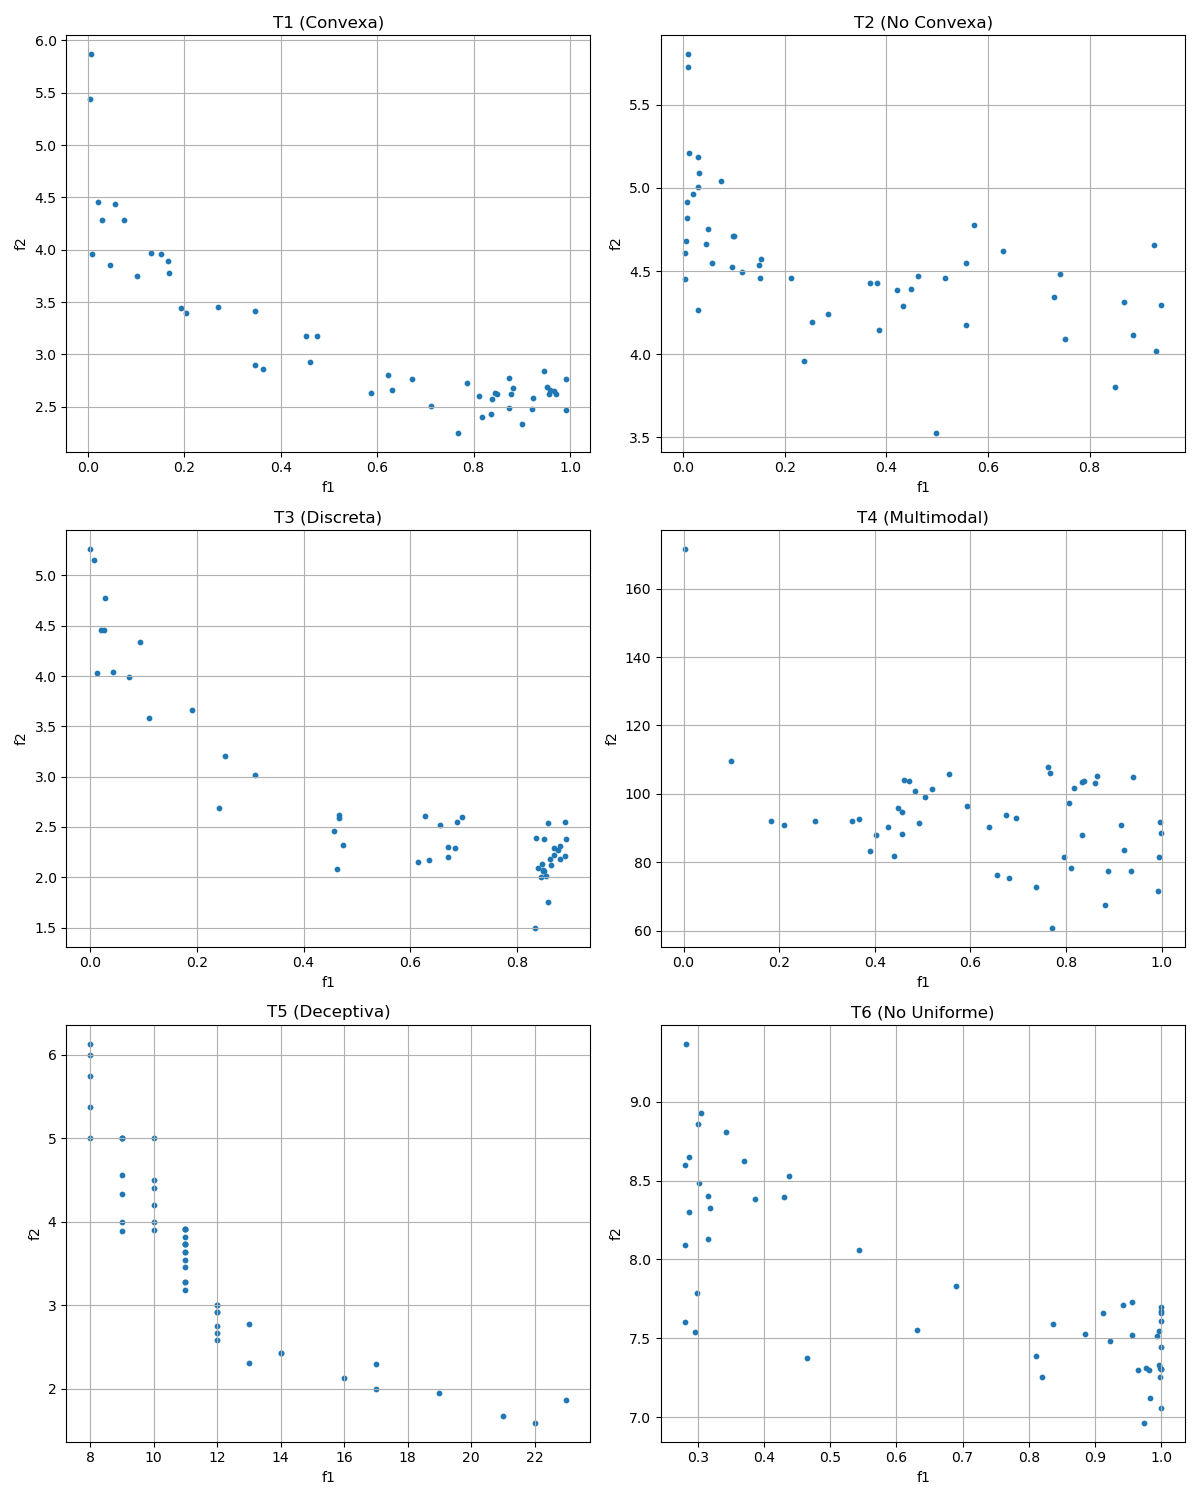
\includegraphics[width=0.9\textwidth]{img/resultados_bbo_3x2.png}
    \caption{Frentes de Pareto aproximados obtenidos por BBO-SOEA para las seis funciones de prueba T1 a T6.}
    \label{fig:resultados_bbo_3x2}
\end{figure}

Mediante la realización de esta práctica, hemos comprendido en profundidad el algoritmo y la analogía que tiene inspirada en la naturaleza y la biología. La implementación de las funciones de prueba ha sido importante para poder ver el rendimiento de este algoritmo en diferentes problemas y poder comprender en qué casos funciona mejor. Ver como BBO se enfrenta a estos problemas \textit{benchmark} nos ha ayudado a comprender y relacionar la teoría vista en clase con la práctica computacional.

\pagebreak

% ANTS
\section{Sistema de hormigas Elitista}



\subsection{Introducción}

Uno de los problemas más estudiados por los etólogos ha sido entender cómo animales con capacidades visuales
limitadas, como las hormigas, logran establecer rutas eficientes desde su colonia para conseguir recursos y volver.
Se ha descubierto que la forma más usual para comunicar información entre los individuos sobre los caminos, 
y que se usa para decidir a dónde ir, se basa en el rastro de feromonas.
El movimiento de hormigas deposita esta sustancia en el suelo, marcando el sendero.
Este mecanismo genera un proceso de retroalimentación positiva: de tal forma que cuanto más sigan las hormigas 
un rastro, más atractivo se vuelve ese rastro para ser seguido. 
En concreto, este comportamiento colectivo se caracteriza porque la probabilidad de que una hormiga escoja 
un camino aumenta en función del número de individuos que ya han transitado esa misma ruta.

\subsection{Sistema de Hormigas}

En primer lugar vamos a utilizar el problema del viajante de comercio (TSP) como caso de estudio para
implementar nuestro sistema de hormigas elitista. 
El TSP es un problema clásico de optimización combinatoria que busca encontrar la ruta más corta 
que visite un conjunto de ciudades exactamente una vez y regrese a la ciudad de origen.

Dado un conjunto de n ciudades, denominamos $d_{ij}$ a la longitud del camino entre la ciudades i y j,
que suele ser la distancia euclídea. Este conjunto de ciudades y caminos viene representado por un grafo (N, E),
donde N es el conjunto de nodos (ciudades) y E el conjunto de aristas (caminos entre ciudades).

Denominamos $b_i(t)$ el número total de hormigas en la ciudad i en el tiempo t y $m = \sum_{i=1}^{n} b_i(t)$ 
el número total de hormigas en el tiempo t.
Cada hormiga dispone de las siguientes características:
\begin{itemize}
    \item Escoge la ciudad siguiente con una probabilidad, que es función de la cantidad de feromona en el camino y de la distancia a la ciudad siguiente.
    \item Obligamos a que realice recorridos válidos, prohibiendo las transiciones a pueblos ya visitados hasta que se complete un recorrido, mediante una lista tabú.
    \item Cuando se completa un recorrido, deposita una sustancia llamada rastro en cada arista visitada.
\end{itemize}

Sea $\tau_{ij}(t)$ la cantidad de feromona en el camino entre las ciudades i y j en el tiempo t.
Cada hormiga en el tiempo t, debe escoger la siguiente ciudad, donde estará en tiempo t+1.
Por lo tanto, si llamamos a una iteración del algoritmo a los m movimientos realizados por las m hormigas en el intervalo (t, t+1), 
entonces cada n iteraciones del algoritmo, cada hormiga ha completado un recorrido, lo que denominaremos ciclo.

En cada ciclo la intensidad del camino se actualiza de la siguiente forma:
\begin{equation}
    \tau_{ij}(t+n) = \rho \cdot \tau_{ij}(t) + \Delta \tau_{ij}
\end{equation}
donde $0 < \rho < 1$ es un coeficiente tal que $1 - \rho$ representa la evaporación del camino entre t y t+n, y
\begin{equation}
   \Delta \tau_{ij} = \sum_{k=1}^{m} \Delta \tau_{ij}^k
\end{equation}
donde $\Delta \tau_{ij}^k$ es la cantidad por unidad de longitud de feromona que la hormiga k deposita en el camino entre las ciudades i y j, 
entre el tiempo t y t+n.
Esta cantidad se define como:
\begin{equation}
    \Delta \tau_{ij}^k = \begin{cases}
    Q / L_k & \text{si la hormiga } k \text{ utiliza el camino } (i, j) \text{ en su recorrido}\\
    0 & \text{en otro caso}
    \end{cases}
\end{equation}
donde Q es una constante y $L_k$ la longitud del recorrido realizado por la hormiga k.

Con el objetivo de satisfacer la restricción de que cada hormiga debe visitar todas las n diferentes ciudades, asociamos a cada hormiga
una lista tabú que almacena las ciudades ya visitadas por esa hormiga.
Cuando se completa un ciclo, la lista tabú se utiliza para calcular la solución actual de cada hormiga.
Luego, la lista se vacía y cada hormiga comienza un nuevo ciclo.

Llamamos visibilidad, $n_{ij}$, a la distancia inversa entre las ciudades i y j, $\frac{1}{d_{i,j}}$. 
Esta cantidad no se modifica durante la ejecución del algoritmo y representa la información heurística disponible para las hormigas.

Definimos la probabilidad de transición de una ciudad i a una ciudad j para la hormiga k en el tiempo t como:
\begin{equation}
    p_{ij}^k = \begin{cases}
    \frac{[\tau_{ij}(t)]^{\alpha} \cdot [n_{ij}]^{\beta}}{\sum_{l \in \text{allowed}_k} [\tau_{il}(t)]^{\alpha} \cdot [n_{il}]^{\beta}} & \text{si } j \in \text{allowed}_k\\
    0 & \text{en otro caso}
    \end{cases}
    \label{eq}
\end{equation}
donde $\text{allowed}_k$ es el conjunto de ciudades que la hormiga k no ha visitado aún, y $\alpha$ y $\beta$ son parámetros que controlan la
importancia relativa entre la feromona y la visibilidad.
Por lo tanto, esta probabilidad es un equilibrio entre la visibilidad, que indica que se deben elegir las ciudades más cercanas con mayor probabilidad,
y la intensidad del rastro en el tiempo t, que indica que si en la arista (i, j) ha habido mucho tráfico, entonces ese camino es más atractivo.

\subsection{Algoritmo}

El algoritmo comienza con una fase de inicialización, donde las hormigas se posicionan en diferentes ciudades y se establece la intensidad inicial de feromona en cada arista del grafo
mediante $\tau_{ij}(0)$. Inicializamos el primer elemento de la lista tabú de cada hormiga con la ciudad donde se encuentra.

Luego, cada hormiga se moverá desde la ciudad i a la ciudad j según la probabilidad de transción y tras n iteraciones todas las hormigas habrán completado un ciclo y sus listas tabú contendrán un recorrido completo.
En este punto, para cada hormiga k se actualiza $L_k$ y la intensidad de feromona en cada arista del grafo según la fórmula dada anteriormente.
Además, se guarda el camino más corto encontrado, $min_k L_k, \quad k = 1,...,m$.
Este proceso se repite hasta que se cumple un criterio de parada, como alcanzar un número máximo de ciclos, $NC_{MAX}$ o todas las hormigas convergen a la misma solución.

Formalmente, el algoritmo se puede describir con los siguientes pasos:
\begin{enumerate}
    \item Inicialización: \\
    \hspace*{0.25cm} Definimos t := 0. \\
    \hspace*{0.25cm} Definimos NC := 0. \\
    \hspace*{0.25cm} Para cada arco (i, j) definimos la intensidad $\tau_{ij}(0) = c$ y $\Delta \tau_{ij} = 0$. \\
    \hspace*{0.25cm} Colocar las m hormigas en los n nodos.
    \item Sea s := 1. \\
    Para k = 1 hasta m hacer \\
    \hspace*{0.25cm} Colocar la ciudad inicial de la hormiga k en la lista tabú, $tabu_k(s)$. 

    \item Repetir hasta que la lista tabú se complete: \\
    Definimos s := s+1 \\
    Para k = 1 hasta m hacer \\
    \hspace*{0.25cm} Elegir la ciudad j a la que moverse con probabilidad $p_{ij}^k(t)$. \\
    \hspace*{0.25cm} Mover la hormiga k a la ciudad j. \\
    \hspace*{0.25cm} Colocar la ciudad j en la lista tabú, $tabu_k(s)$. 
    
    \item Para k = 1 hasta m hacer \\
    \hspace*{0.25cm} Mover la hormiga k de $tabu_k(n)$ a $tabu_k(1)$. \\
    \hspace*{0.25cm} Calcular la longitud del recorrido descrito por la hormiga k, $L_k$. \\
    \hspace*{0.25cm} Actualizar el camino más corto encontrado. \\
    \hspace*{0.25cm} Para cada arco (i, j) del grafo hacer \\
    \hspace*{0.25cm} Para k = 1 hasta m hacer 
    \begin{equation*}
        \Delta \tau_{ij}^k = \begin{cases}
        Q / L_k & \text{si } (i, j) \in \text{ciclo descrito por } tabu_k \\
        0 & \text{en otro caso}
        \end{cases}
    \end{equation*}

    \hspace*{0.25cm} $\Delta \tau_{ij} := \Delta \tau_{ij} + \Delta \tau_{ij}^{k}$

    \item Para cada arco (i, j) calcular $\tau_{ij}(t+n) = \rho \cdot \tau_{ij}(t) + \Delta \tau_{ij}$. \\
    Definir t := t + n. \\
    Definir NC := NC + 1. \\
    Para cada arco (i, j) definir $\Delta \tau_{ij} := 0$. 

    \item Si $(NC < NC_{MAX})$ y no todas las hormigas han convergido a la misma solución \\
    entonces \\
    \hspace*{0.25cm} Vaciar todas las listas tabú. \\
    \hspace*{0.25cm} Ir al paso 2. \\
    sino \\
    \hspace*{0.25cm} Imprimir el ciclo más corto encontrado. \\
    \hspace*{0.25cm} Parar.

\end{enumerate}

\subsubsection{Estrategia elitista}

Para mejorar el rendimiento del algoritmo, implementamos una estrategia elitista. 
Para ello añadimos al camino de cada arco del mejor ciclo la cantidad $e \cdot Q/L^{*}$, donde e es el número de hormigas elitistas y $L^{*}$ la longitud del mejor ciclo encontrado hasta el momento.
De esta forma, se refuerza el camino del mejor ciclo, acelerando la convergencia del algoritmo.
\subsection{Implementación}

Para validar el funcionamiento del Sistema de Hormigas Elitista, se ha realizado una implementación práctica en lenguaje Python. El desarrollo parte de los requisitos establecidos en el enunciado de la Práctica 9, evolucionando desde la resolución del problema base hacia una propuesta experimental multi-objetivo.

\subsubsection{Descripción del Problema y Entorno}

El problema a resolver es el \textbf{Problema de Asignación Generalizado} descrito en el enunciado de la práctica. Este escenario plantea la necesidad de asignar un conjunto de $N=4$ tareas, denotadas como $T_i$ ($i=\{1,..,4\}$), a un conjunto de $M=5$ operarios, denotados como $O_j$ ($j=\{1,..,5\}$).

El modelo está sujeto a las siguientes restricciones y parámetros definidos en la documentación:
\begin{itemize}
    \item \textbf{Restricción de Unicidad:} Cada tarea debe ser realizada por un único operario.
    \item \textbf{Restricción de Capacidad:} Aunque un operario puede realizar múltiples tareas, la suma de los tiempos requeridos por estas ($r_i$) no puede exceder el tiempo total disponible de dicho operario ($d_j$).
    \item \textbf{Función de Coste:} Existe un coste $c_{ij}$ asociado a que el operario $j$ realice la tarea $i$.
\end{itemize}

El objetivo fundamental estipulado es encontrar la asignación válida que minimice el coste total. No obstante, en esta implementación hemos decidido ir un paso más allá de lo solicitado: además de resolver el problema mono-objetivo original, hemos introducido artificialmente un segundo objetivo de optimización (equilibrio de carga) para testar la flexibilidad del algoritmo en entornos multi-objetivo.

Los datos utilizados se corresponden fielmente con la tabla proporcionada en el enunciado, modelados computacionalmente mediante \texttt{NumPy}:

\begin{equation}
C_{ij} (\text{Costes}) = \begin{pmatrix}
2 & 3 & 4 & 1 \\
3 & 2 & 3 & 2 \\
2 & 2 & 1 & 2 \\
3 & 3 & 3 & 3 \\
2 & 1 & 2 & 2
\end{pmatrix}
\end{equation}

\begin{equation}
r_{i} (\text{T. Requerido}) = [3, 2, 2, 3], \quad
d_{j} (\text{T. Disponible}) = [4, 5, 3, 4, 4]
\end{equation}

\subsubsection{Enfoque mono-objetivo: (Elitist Ant System)}

En esta primera fase, nos ceñimos estrictamente al objetivo del enunciado: minimizar el coste total ($f_1 = \sum c_{ij}$). Se implementó el algoritmo descrito en el apartado 3.3, definiendo la información heurística $\eta_{ij}$ como la inversa del coste ($1/c_{ij}$), tal que las hormigas tiendan a escoger las asignaciones más económicas. Se aplicó la estrategia elitista para reforzar el mejor camino global encontrado en cada iteración.

\subsubsection{Extensión multi-objetivo (MOACO y MAS)}

Para extender la práctica y analizar el comportamiento de las metaheurísticas ante conflictos de objetivos, definimos un segundo objetivo no presente en el enunciado original:
\begin{itemize}
    \item \textbf{Objetivo 1 ($f_1$):} Minimizar Coste Total (Objetivo original).
    \item \textbf{Objetivo 2 ($f_2$):} Minimizar el Desequilibrio de Carga (Desviación típica del tiempo de trabajo entre operarios).
\end{itemize}

Se implementaron dos variantes para resolver este problema bi-objetivo:
\begin{enumerate}
    \item \textbf{Simple MOACO:} Utiliza un archivo externo para almacenar el Frente de Pareto.
    \item \textbf{MAS (Multi-Objective Ant System):} Asigna pesos variables $\lambda$ a cada hormiga para equilibrar la importancia de ambos objetivos.
\end{enumerate}
\subsubsection{Resultados Experimentales}

El primer análisis se realizó utilizando estrictamente las matrices de costes y tiempos proporcionadas en el enunciado de la Práctica 9. Tras ejecutar tanto la variante Mono-objetivo como las variantes Multi-objetivo (MOACO y MAS), se observó un fenómeno de convergencia unificada.

\begin{itemize}
    \item \textbf{Solución Obtenida:} Todos los algoritmos convergieron a la misma solución global:
    \begin{itemize}
        \item Coste Total ($f_1$): \textbf{6} (Mínimo teórico).
        \item Desequilibrio ($f_2$): \textbf{1.0954} (Desviación típica).
    \end{itemize}
\end{itemize}

Este comportamiento se debe a la topología específica de los datos de entrada. En esta instancia del problema GAP, los objetivos resultaron ser no conflictivos. La asignación de tareas a los operarios más eficientes en costes minimizando $f_1$ generó, de manera colateral, una distribución de carga que no violaba las restricciones y mantenía un desequilibrio bajo. Al no existir conflicto entre ahorrar dinero y equilibrar carga, el Frente de Pareto teórico colapsó en un único punto dominante, impidiendo visualizar una curva de compromiso trade-off real.


Uno de los aspectos críticos en la validación del algoritmo es asegurar que la solución encontrada no solo minimiza la función objetivo, sino que respeta estrictamente las restricciones de capacidad del problema GAP.A primera vista, una inspección de la matriz de costes $C_{ij}$ sugeriría que el coste mínimo teórico podría ser $f_1 = 5$. Este valor se obtiene aplicando una estrategia \textit{greedy}, seleccionando el mínimo absoluto de cada tarea sin considerar el consumo de recursos. Sin embargo, como se ilustra en la Figura \ref{fig:gap_analysis}, esta combinación es inviable:

\begin{figure}[h]
    \centering
    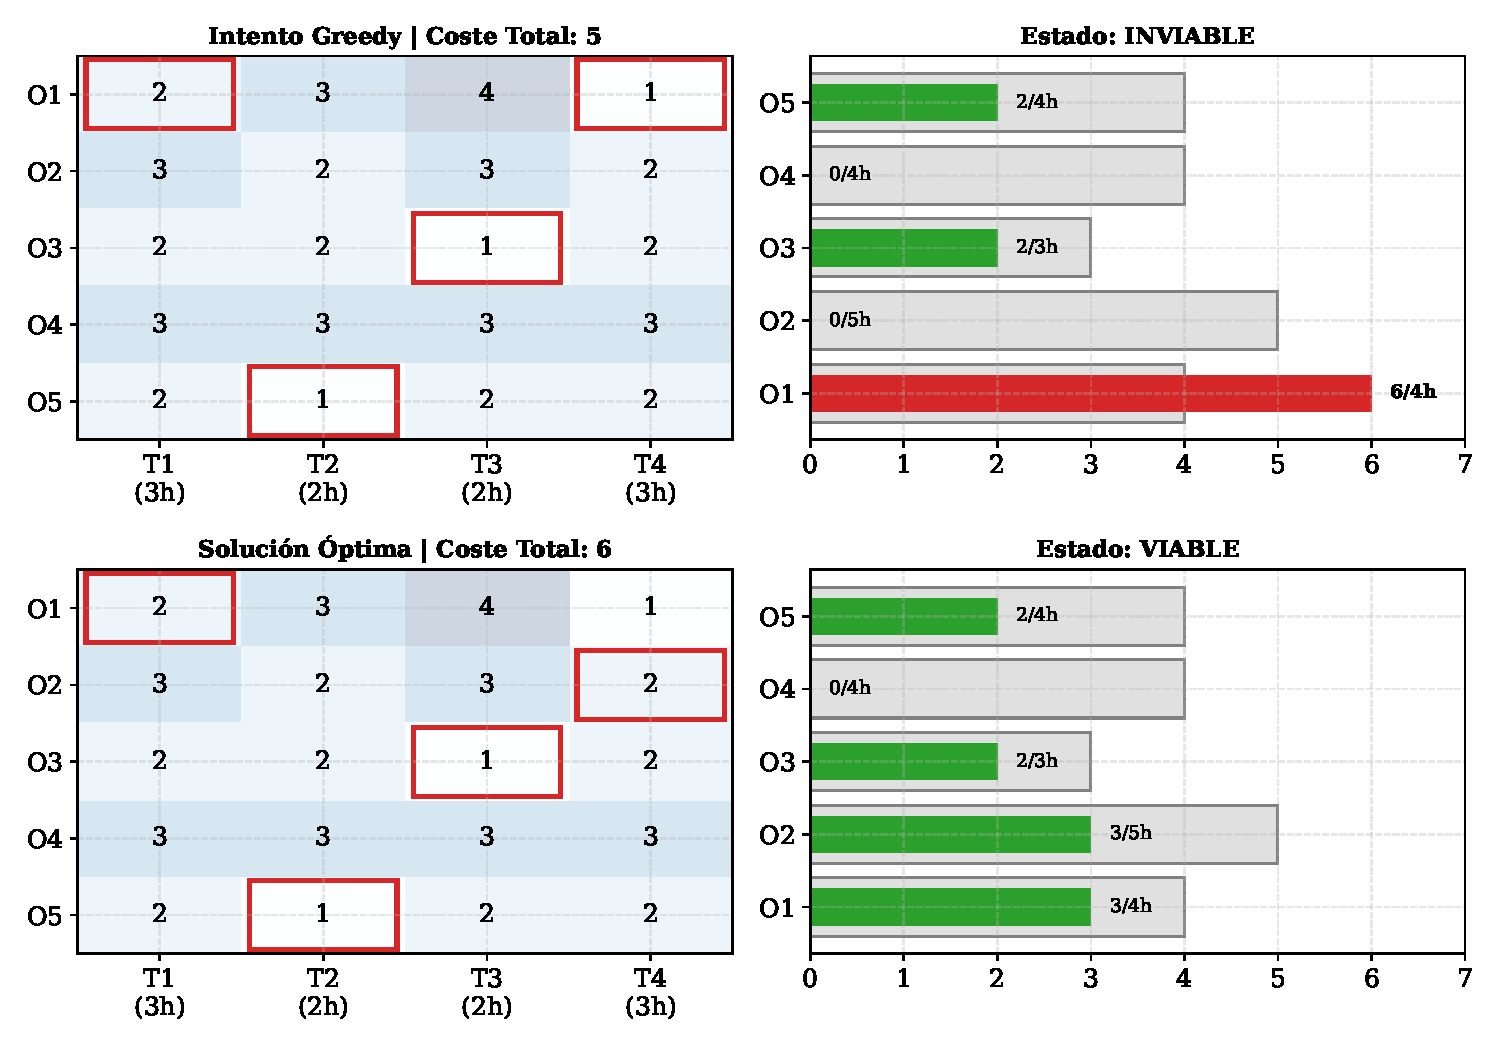
\includegraphics[width=1.0\textwidth]{img/explicacion_sol_ants.pdf}
    \caption{Comparativa entre la selección Greedy y la solución óptima. Sumando los mínimos absolutos viola la capacidad del $O_1$.}
    \label{fig:gap_analysis}
\end{figure}

Por lo tanto, la solución mínima viable de este problema es $f_1 = 6$ tan y como han indicado los tres algoritmos implementados en la práctica. A continuación decidimos crear otro escenario donde las habilidades de los operarios eran menos regulares dando a lugar a un frente de pareto para los algoritmos multiobjetivo.

\textbf{Validación Adicional: Escenario de Conflicto}

Dado que los datos originales no permitían apreciar la capacidad del algoritmo para gestionar objetivos contrapuestos, se diseñó un segundo escenario experimental. El objetivo fue forzar la aparición de un Frente de Pareto real modificando los datos de entrada para generar un conflicto explícito entre Coste y Equilibrio.
Se definió un problema con $N=8$ tareas y $M=3$ operarios con perfiles extremos:
\begin{itemize}
    \item \textbf{Operario 1 (barato):} Coste muy bajo ($c=1$) pero alta probabilidad de saturación.
    \item \textbf{Operario 2 (medio):} Coste moderado ($c=4$).
    \item \textbf{Operario 3 (caro):} Coste alto ($c=8$), su uso es necesario para equilibrar la carga pero penaliza el coste.
\end{itemize}

Al ejecutar el algoritmo MOACO sobre este nuevo conjunto de datos, se obtuvo un conjunto de soluciones no dominadas diverso, tal como se muestra en la Figura \ref{fig:pareto}.

\begin{figure}[H]
    \centering
    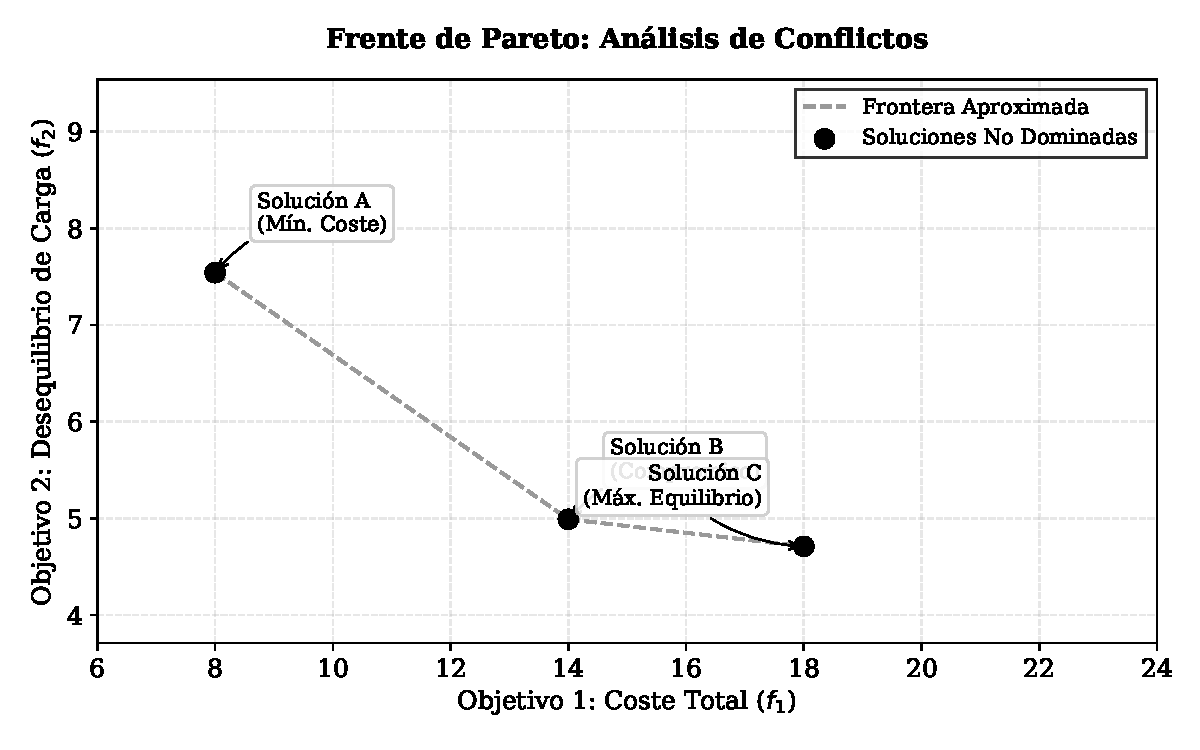
\includegraphics[width=0.7\textwidth]{img/ants_results.pdf}
    \caption{Frente de Pareto obtenido en el escenario de conflicto. Se observa la curva de compromiso entre el Coste Total y el Desequilibrio de Carga.}
    \label{fig:pareto}
\end{figure}

A diferencia del caso anterior, aquí se observan claramente tres regiones de decisión:
\begin{enumerate}
    \item \textbf{Región de mínimo coste ($f_1 \approx 8$):} El algoritmo asigna casi todo al Operario 1. El coste es mínimo, pero el desequilibrio ($f_2$) se dispara por encima de 7.5.
    \item \textbf{Región de compromiso ($f_1 \approx 14$):} Se empieza a derivar trabajo al Operario 2. El coste sube, pero el desequilibrio mejora notablemente.
    \item \textbf{Región de máximo equilibrio ($f_1 \approx 18$):} Se utiliza al Operario 3. Es la opción más cara, pero logra la distribución de trabajo más equitativa posible ($f_2 < 4.8$).
\end{enumerate}

La segunda fase experimental valida la robustez de la implementación, demostrando su capacidad para mantener la diversidad poblacional y hallar soluciones de compromiso en escenarios de conflicto real, superando así las limitaciones observadas en los datos originales. Por otro lado, el análisis de la Figura \ref{fig:gap_analysis} justifica estructuralmente el resultado obtenido: mientras que una estrategia greedy alcanzaría un coste teórico de 5 a expensas de violar la capacidad del Operario 1 (quien recibiría 6 horas de carga frente a sus 4 disponibles), el sistema converge correctamente hacia el óptimo factible de coste 6, priorizando el cumplimiento estricto de las restricciones mediante la reasignación eficiente de recursos.
\pagebreak

% FANS
\input{fans.tex}
\pagebreak

% Conclusiones
\section{Conclusiones}

La realización de esta práctica ha permitido profundizar en el comportamiento y la aplicabilidad de diferentes de diferentes metaheurísticas.

En lo relativo al algoritmo de \textbf{Optimización Basada en Biogeografía (BBO)}, su implementación nos ha resultado notablemente intuitiva. El mayor valorq que hemos aprendido de esta fase ha sido la experimentación con las funciones de prueba $T_1$ a $T_6$; someter al algoritmo a estos entornos controlados nos ha permitido comprender cómo se comporta la búsqueda ante Frentes de Pareto con geometrías muy diversas (convexas, cóncavas o discontinuas), revelando la gran utilidad de estos \textit{benchmarks} estándar para validar la robustez de cualquier optimizador.

Por su parte, el \textbf{Sistema de Hormigas Elitista} ha destacado por la elegancia y originalidad de su inspiración biológica basada en el rastro de feromonas. Inicialmente, la resolución del problema mono-objetivo planteado en el enunciado nos pareció sencilla debido a la eficacia del algoritmo. Es por esto que decidimos explorar los límites de la técnica, extendiendo la implementación hacia una variante multi-objetivo. Esta decisión aumentó la complejidad técnica y nos permitió observar cómo funcionan las soluciones de compromiso en problemas combinatorios.

En cuanto a la metaheurística \textbf{FANS (Fuzzy Adaptive Neighborhood Search)}, lo más reseñable ha sido comprender su gran polivalencia. El uso de lógica difusa para evaluar las soluciones brinda al algoritmo de una flexibilidad única, permitiéndole adaptarse a un gran abanico de problemas de optimización sin necesidad de redefinir rígidamente los criterios de aceptación, lo cual lo convierte en una herramienta sumamente versátil en comparación con métodos de búsqueda local más tradicionales.

Finalmente, desde una perspectiva técnica, el desarrollo de estos algoritmos en Python ha supuesto un aprendizaje muy valioso. Hemos comprobado la existencia de una gran cantidad de repositorios de código abierto y librerías dedicadas a la computación evolutiva. La disponibilidad de estas referencias no solo acelera el proceso de implementación, sino que permite contrastar nuestras soluciones con estándares de la comunidad, facilitando la detección de errores y mejorando de la eficiencia computacional de los algoritmos.
\pagebreak

%%% BIBLIOGRAFIA

\bibliographystyle{IEEEtran}
\nocite{*}
\renewcommand{\refname}{Bibliografía}
\bibliography{./referencias.bib} 

\end{document}